%Version 3.1 December 2024
%% Δ-IRIS interpretability paper — Nature-style Article (Introduction/Results/Discussion/Methods).
%% Compile: tectonic sn-article.tex   (requires sn-jnl.cls + sn-mathphys-num.bst alongside)
%% Supplementary Information: sn-supplementary.tex

\documentclass[pdflatex,sn-mathphys-num]{sn-jnl}% Math and Physical Sciences Numbered Reference Style

\usepackage{graphicx}%
\usepackage{multirow}%
\usepackage{amsmath,amssymb,amsfonts}%
\usepackage{amsthm}%
\usepackage{mathrsfs}%
\usepackage[title]{appendix}%
\usepackage{xcolor}%
\usepackage{textcomp}%
\usepackage{manyfoot}%
\usepackage{booktabs}%
\usepackage{algorithm}%
\usepackage{algorithmicx}%
\usepackage{algpseudocode}%
\usepackage{listings}%

\theoremstyle{thmstyleone}%
\newtheorem{theorem}{Theorem}%
\newtheorem{proposition}[theorem]{Proposition}%

\theoremstyle{thmstyletwo}%
\newtheorem{example}{Example}%
\newtheorem{remark}{Remark}%

\theoremstyle{thmstylethree}%
\newtheorem{definition}{Definition}%

\raggedbottom

% Notation shortcuts
\newcommand{\deltairis}{$\Delta$-IRIS}
\newcommand{\code}[2]{(s_{#1},c_{#2})}
\newcommand{\achname}[1]{\texttt{#1}}

\begin{document}

\title[From Codes to Causes, and Where the Chain Breaks]{From Codes to Causes---and Where the Chain Breaks: A Causal Interpretability Audit of Quantized Delta Representations in a Transformer World Model}

\author[1]{\fnm{Runze} \sur{Xia}}\email{r.xia2@lancaster.ac.uk}
%% NOTE: confirm R.J.'s email/ORCID before submission.
\author*[1]{\fnm{Richard} \sur{Jiang}}\email{r.jiang2@lancaster.ac.uk}

\affil*[1]{\orgname{Lancaster University}, \orgaddress{\city{Lancaster}, \postcode{LA1 4YW}, \country{United Kingdom}}}

\abstract{World-model agents compress dynamics into discrete latent codes, but whether those codes are interpretable and causally meaningful is untested. We audit \deltairis{}, a transformer world-model agent on Crafter that acts inside its own imagination, separating three levels at which a direction can be causal: it can \emph{decode} a concept, \emph{write} its next codes, or \emph{drive} behaviour---with a dissociation at each seam. The context-aware ``delta'' codes form an event-specific vocabulary, detecting events up to $708\times$ above chance. Supervised probe directions decode near-perfectly yet are not what the model writes through; an unsupervised sparse-autoencoder direction is. But that write does not drive: ablating it erases an event's code without changing imagined behaviour or return, because a heads-up-display shortcut lets later steps re-derive it from the frame. The model's imagination does not enforce its own tech tree---a reliability caveat for planning---and decodability must not be equated with mechanism.}

\keywords{world models, interpretability, reinforcement learning, discrete representations, sparse autoencoders, causal analysis}

\maketitle

% ===================== INTRODUCTION (no heading) =====================
Model-based reinforcement-learning agents increasingly learn inside their own imagination: a learned \emph{world model} predicts future observations, rewards and terminations, and the policy is optimised largely on imagined trajectories~\cite{worldmodels2018,simple2020,muzero2020,dreamerv3}. A prominent family tokenizes observations into discrete latent codes and models dynamics autoregressively with a transformer~\cite{iris2023}. The recent \deltairis{} agent~\cite{deltairis2024} refines this with \emph{context-aware tokenization}: rather than encoding each frame in isolation, its tokenizer encodes the \emph{transition} $(x_t, a_t, x_{t+1})$ into four discrete codes, and its decoder reconstructs $x_{t+1}$ with direct access to $(x_t, a_t)$. The codes are thereby pressured to carry only what is \emph{new}---a compressed description of the frame-to-frame delta.

This suggests an interpretability hypothesis: if codes describe changes, and meaningful events are changes, the codebook should be an \emph{event vocabulary}---discrete, enumerable, potentially human-legible. Whether this holds, and more importantly whether such codes (or representations derived from them) are \emph{causally} implicated in the model's predictions rather than merely correlated with events, has to our knowledge not been tested. The distinction matters because high decoding accuracy does not imply a representation is used~\cite{belinkov2022probing,hewitt2019control,amnesic2021}: interpretability claims about world models should climb from description, through information, to intervention before they are believed.

We test the hypothesis on one fully trained \deltairis{} agent (one seed, one environment) on Crafter~\cite{crafter2022}, a procedurally generated survival game with 22 ground-truth achievement signals that fire at known timesteps---ideal event labels. We audit it in three tiers of evidentiary strength: \emph{descriptive} (codebook statistics and code--event association over the full $10^7$-step replay buffer); \emph{informational} (linear probes and concept activation vectors~\cite{tcav2018} across the tokenizer, the convolutional frame encoder and every transformer block, plus a TopK sparse autoencoder~\cite{gao2024topk,sae2024} on the residual stream); and \emph{interventional} (projection ablation on single-step prediction and inside the multi-step imagination loop, multi-direction subspace ablation, and activation patching~\cite{vig2020causal,rome2022}). This audit is, to our knowledge, among the first systematic interpretability studies of the discrete \emph{transition} vocabularies learned by IRIS-family world models; it complements interpretability-by-architecture approaches~\cite{spartan2025} and post-hoc analyses of game-playing and next-token sequence models, where probe-decoded world-state directions are causally steerable~\cite{li2023othello,nanda2023othello,spies2025maze,butkus2025causal} and where the residual stream is found to encode structured belief-state geometry~\cite{shai2024belief}.

Four findings result. (i) The delta codes form a highly event-specific vocabulary, and a controlled baseline indicates the \emph{delta conditioning} is the primary factor driving this specialisation. (ii) A ``heads-up-display (HUD) shortcut'': probes suggest the transformer tracks episodic state, until a control representation---the frame encoder alone---matches it, because Crafter renders state on screen. (iii) A \emph{read--write asymmetry}---decodable from a representation is not the same as used by it: supervised probe directions decode at near-perfect AUROC yet have negligible causal effect, while an unsupervised dictionary direction is causally load-bearing inside imagination; the asymmetry persists under rank-16 subspace ablation. (iv) Next-code prediction is causally \emph{quasi-Markovian}---driven by the current frame and action, not by the deeper history. Beyond the specific results, the audit (Fig.~\ref{fig:overview})---descriptive association, probing with shortcut controls, dictionary learning, then intervention inside imagination---is a transferable methodology for interrogating discrete world-model representations.

\begin{figure}[t]
\centering
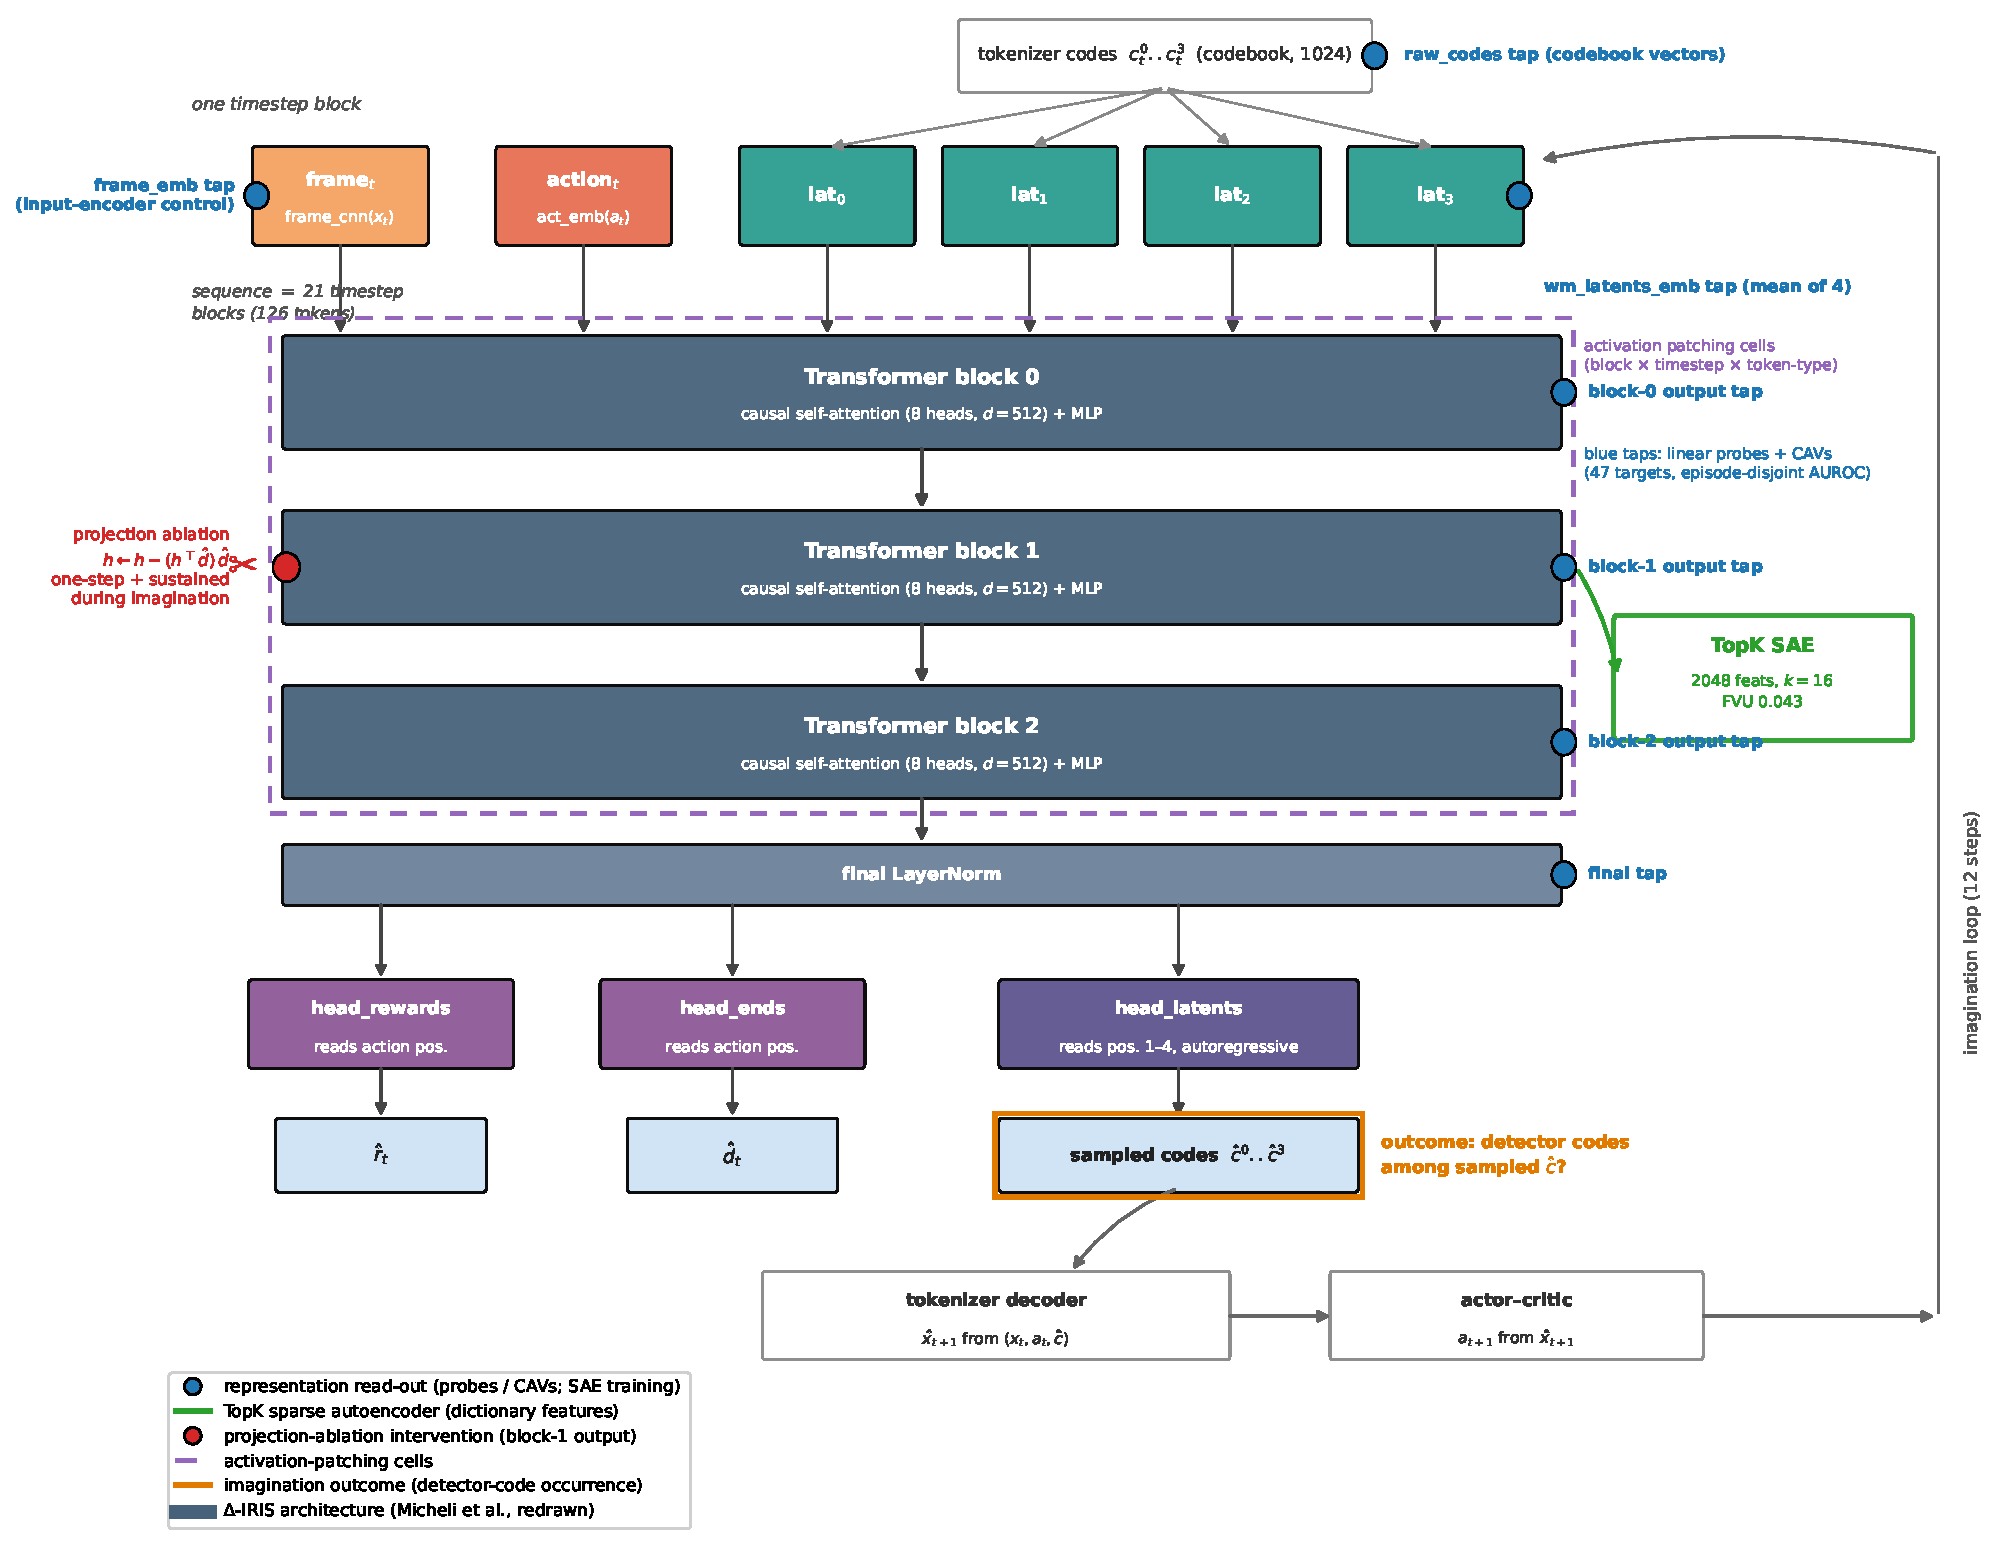
\includegraphics[width=\textwidth]{figures/audit_overview.pdf}
\caption{\textbf{Overview of the audit.} Grey-blue: the \deltairis{} world model of Micheli et al.~\cite{deltairis2024} (redrawn). Coloured: our instrumentation---blue, the seven probe/CAV read-out points including the \textsf{frame\_emb} control; green, the TopK sparse autoencoder on the block-1 output; red, the projection-ablation point; purple, the activation-patching cell grid; orange, the imagination-loop outcome.}\label{fig:overview}
\end{figure}

% ===================== RESULTS =====================
\section{Results}\label{sec:results}

\subsection{Delta codes form an event vocabulary}\label{sec:res-vocab}
Re-encoding the agent's entire replay buffer ($29{,}136$ episodes; $9{,}980{,}073$ transitions) shows no codebook collapse---all $1024$ codes are used---but heavily concentrated usage (per-slot entropy $5.3$--$6.0$ of $10$ bits; the single code 29 dominates every slot and marks ``no change in this quadrant'') (Supplementary Fig.~S1). The informative vocabulary lives in the long tail. Computing, for every (slot, code, achievement) cell, the conditional probability $P(u^i \mid c^k{=}j)$ and its lift over base rate, the strongest codes are bona-fide event detectors: $\code{3}{75}$ co-occurs with \achname{collect\_iron} $88\%$ of the time ($708\times$ chance), $\code{3}{938}$ with \achname{place\_plant} at $0.92$ ($543\times$), $\code{2}{707}$ with \achname{collect\_sapling} at $0.90$ (Supplementary Table~S1; all maxima $p<10^{-40}$). Slot~3 hosts $11$ of $18$ per-achievement maxima, indicating specialisation beyond spatial decomposition. Some codes are polysemantic superclasses: $\code{3}{36}$ detects \achname{place\_table}, \achname{make\_wood\_pickaxe} and \achname{make\_wood\_sword}---events whose visual signature (a wooden item appears) is near-identical---a collapse the dictionary later resolves. Combat events are the weakest (\achname{defeat\_skeleton}: best $P{=}0.07$), plausibly because they look heterogeneous.

\textbf{A controlled ablation isolates the delta conditioning.} Is this specialisation due to context-aware delta tokenization specifically, or to discrete quantization in general? Holding the scheme fixed and varying only the conditioning, we train two baselines on the same buffer and run the identical analysis (Methods): a \emph{frame-only ablation} of the \deltairis{} tokenizer (same backbone, codebook and token count, but encoding $x_{t+1}$ alone) and the \emph{original IRIS} frame tokenizer~\cite{iris2023}. The delta codes are $\approx 7\times$ stronger per-event detectors (mean best $P(a\mid c)$ $0.39$ vs $0.06$ and $0.06$; five achievements with a strong $P{\geq}0.5$ detector vs zero), and \deltairis{} dominates on every achievement individually (Fig.~\ref{fig:delta}). Critically the two frame baselines land almost on top of each other despite differing codebook sizes, token counts and architectures: the gap is therefore most plausibly attributable to the delta$+$action conditioning rather than to those incidental differences. Both baselines are healthy tokenizers (PSNR $18.4$/$22.5$, broad codebook use; Methods), so the gap is not a degenerate-baseline artefact.

\begin{figure}[t]
\centering
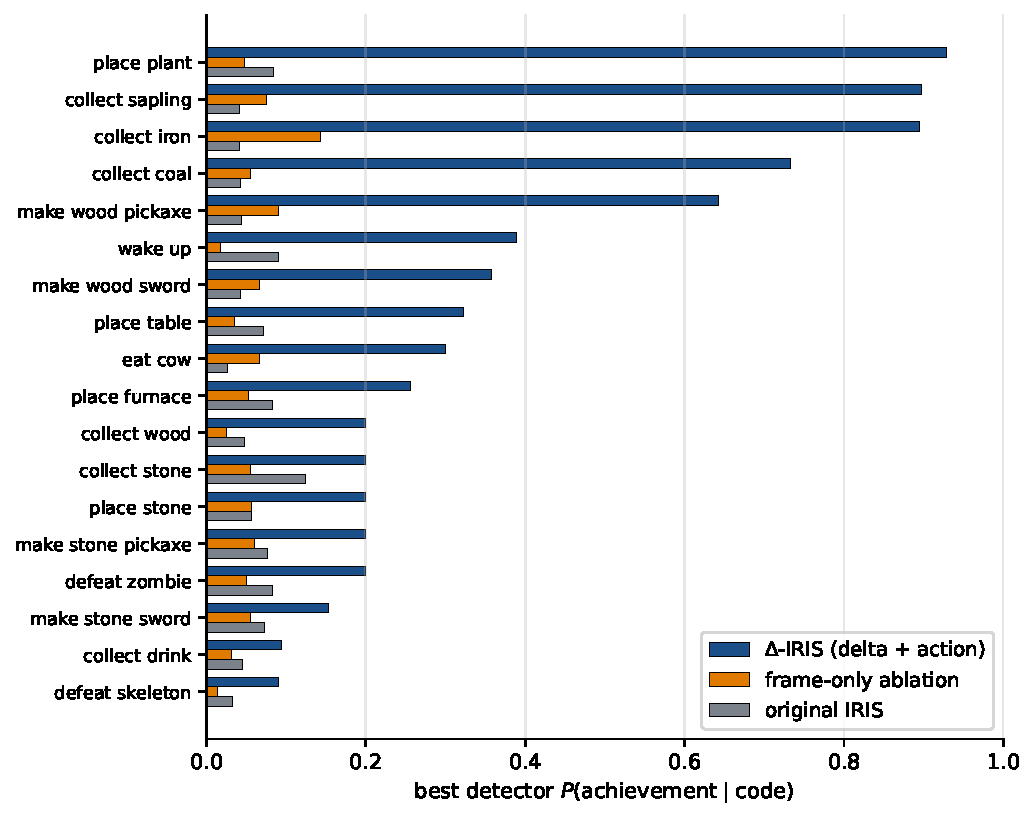
\includegraphics[width=\textwidth]{figures/tokenizer_compare.pdf}
\caption{\textbf{Context-aware delta tokenization is what turns the codebook into an event vocabulary.} Per-achievement best detector $P(\mathrm{achievement}\mid\mathrm{code})$ for the \deltairis{} delta tokenizer, its frame-only ablation, and original IRIS, under identical analysis on a common $150$-episode labelled set. \deltairis{} dominates on every achievement; the frame-only ablation tracks literal IRIS, isolating the gain to the delta$+$action conditioning rather than codebook size, token count or architecture.}\label{fig:delta}
\end{figure}

\subsection{A HUD shortcut masquerades as memory}\label{sec:res-hud}
We train logistic-regression probes for 47 targets on seven representations spanning the tokenizer codes, the world model's convolutional frame embedding (\textsf{frame\_emb}; no transformer), its code embedding, and the four transformer stages, with episode-disjoint splits (Fig.~\ref{fig:probes}; Methods). Just-unlocked events are decodable from the raw codes alone (AUROC $\ge 0.85$ for all 18 measurable achievements, $\ge 0.95$ for 14), confirming the association analysis per-sample. Cumulative state (``has the agent ever collected wood?'') tells a subtler story: near chance from the codes, but excellent ($0.84$--$1.00$) from any transformer block---inviting the conclusion that the transformer maintains episodic memory. The input-encoder control refutes it: \textsf{frame\_emb}, seeing only the current frame, \emph{matches or exceeds every transformer block on 16 of 18} cumulative concepts, a margin that survives paired-bootstrap $95\%$ confidence intervals (Methods). Crafter renders the inventory in the HUD, so cumulative state is written on the screen and one attention step relays it. The one probed target where depth helps monotonically is short-horizon reward anticipation (\textsf{reward\_in\_next\_5}: $0.77\to0.81$ across blocks), the cleanest evidence of what the world model's depth adds. We argue this input-encoder control should be standard when probing pixel-based RL agents, whose observations routinely render persistent state~\cite{atrey2020saliency,hewitt2019control}.

\begin{figure}[t]
\centering
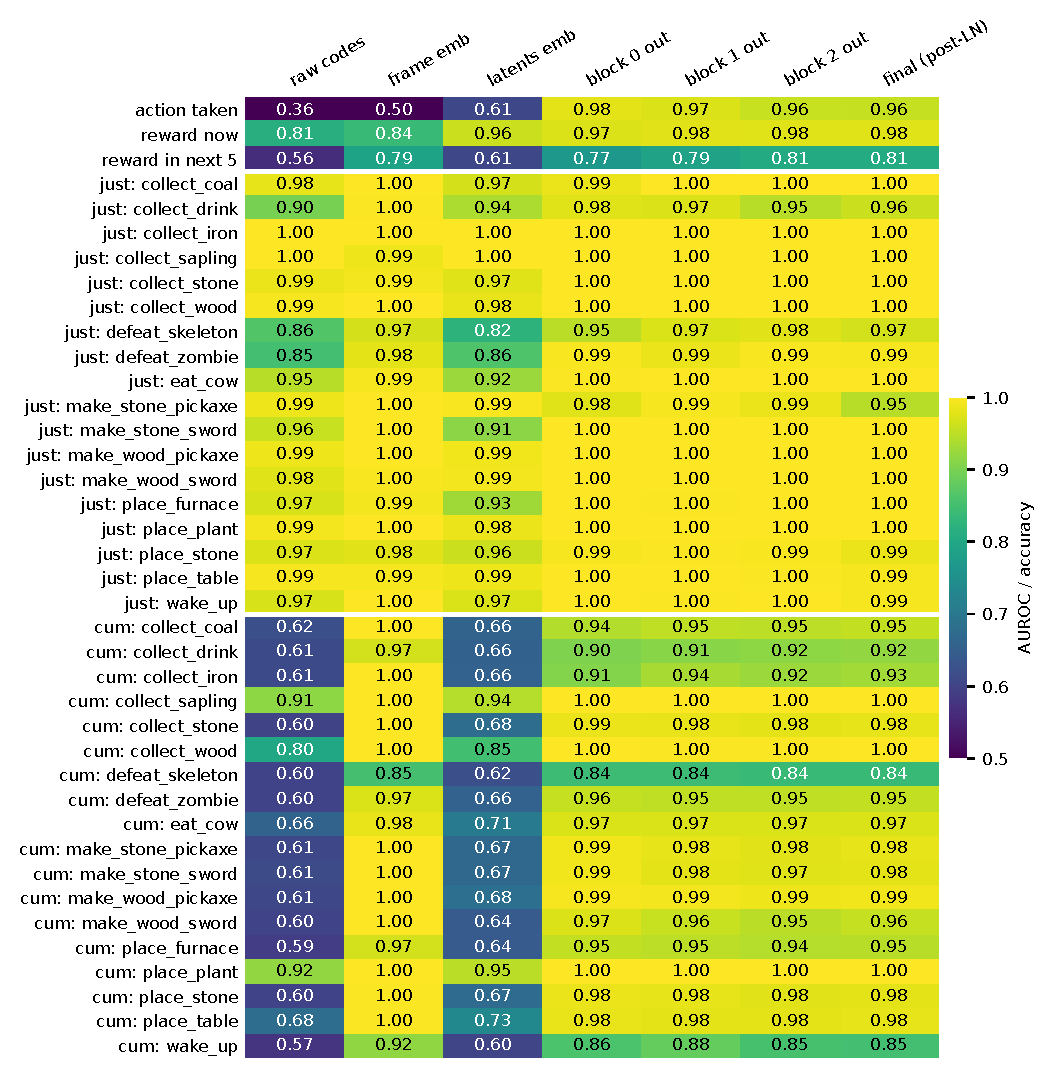
\includegraphics[width=\textwidth]{figures/probe_heatmap.pdf}
\caption{\textbf{The HUD shortcut.} Held-out probe AUROC (accuracy for the 17-way action probe) for 39 measurable targets across seven representations, episode-disjoint, $n{=}81{,}919$ steps. \textsf{frame\_emb} is the input-encoder control (a CNN over the current frame, no transformer). Cumulative-state rows are answered by \textsf{frame\_emb} alone; only \textsf{reward\_in\_next\_5} improves materially with transformer depth.}\label{fig:probes}
\end{figure}

The probe weight vectors are concept activation vectors (CAVs); their pairwise geometry recapitulates Crafter's tech tree (most-aligned pairs are tech-tree neighbours, e.g.\ $\cos(\mathrm{cum}[\achname{collect\_stone}],\mathrm{cum}[\achname{place\_stone}]){=}0.95$), while event and state directions for the same achievement are weakly anti-aligned---though within-episode co-occurrence inflates these alignments, and the intervention tier shows these directions are read-out only. A TopK sparse autoencoder on the block-1 residual stream (Methods) reconstructs well (fraction of variance unexplained $0.043$; zero dead features) and is stable across widths, sparsities, seeds and layers (Methods). It splits the polysemantic code $\code{3}{36}$ into \emph{distinct, individually event-specific features} for \achname{place\_table}, \achname{make\_wood\_pickaxe} and \achname{make\_wood\_sword}: the continuous residual stream retains distinctions the tokenizer's 40-bit bottleneck collapses, and dictionary learning recovers them (Supplementary Table~S2).

\subsection{Decode, write, drive: a dissociation at each seam}\label{sec:res-readwrite}
A representational direction can be causal at three escalating levels: it can let one \emph{decode} a concept, it can be load-bearing for what the model \emph{writes} next (the next-code logits), and it can \emph{drive} what the agent does. We find a dissociation at each boundary---decode without write, and write without drive. Decodability does not imply mechanism. We measure the causal contribution of a direction by projection ablation, $h' = h - (h^\top\hat d)\hat d$, on the block-1 output, contrasting unlock against matched ordinary moments and matched against random directions (Methods). Ablating the matched SAE direction at the unlock step costs up to $+4.85$ nats (\achname{wake\_up}), with \achname{collect\_coal} ($+2.41$) and \achname{collect\_sapling} ($+1.73$) close behind; eight of 18 concepts are significant but the effect concentrates in a handful. Random directions are inert, and an empirical null of 50 random directions confirms specificity (matched effect exceeds the $99$th percentile for \achname{collect\_coal} $z{=}24$, \achname{collect\_sapling} $z{=}9.9$, \achname{make\_stone\_pickaxe} $z{=}3.1$; honest negatives such as \achname{collect\_iron} fall below the null; Supplementary Table~S6). Ablating three steps earlier eliminates the effect entirely---the un-ablated frame embeddings re-inject the information within three steps, the interventional face of the HUD shortcut (Supplementary Fig.~S3).

The stronger test runs inside imagination: after an 8-step burn-in we let the agent dream 12 steps with a direction continuously projected out, and ask whether the event's detector codes are sampled (Fig.~\ref{fig:imag}). For \achname{collect\_wood}, the baseline dreams the wood code at the first imagined step in $100\%$ of rollouts; ablating SAE feature $f_{187}$ reduces this to $0\%$ (Fisher $p<10^{-9}$), while the CAV and a random direction leave it at $100\%$. Removing a single direction in the 512-dimensional residual stream suppresses an event class in imagined futures; decoded filmstrips confirm the event vanishes under the matched ablation but survives an off-target or random one (Supplementary Fig.~S4). Across \emph{all} concepts, ablating the supervised CAV direction---near-perfect AUROC---changes the outcome little (max $|\Delta|{=}0.10$): the directions that suffice to \emph{read} a concept are not the ones the model \emph{writes} through. That is the first seam (decode without write).

\textbf{Write does not drive.} The second seam is that this write does not change behaviour. Because the actor--critic acts on the decoded frames inside imagination, we can ask a question the board-game and maze sequence models structurally cannot, having no downstream policy: does the lesion change what the agent \emph{does}? Using Crafter's tech tree as a ground-truth causal graph (\achname{collect\_wood} gates the wooden-tool tier, which gates the stone tier), the answer is no. Ablating $f_{187}$ drives the wood code from $1.00$ to $0.03$---a $0.97$ swing, so the instrument plainly has power at the upstream node---yet the immediately downstream wooden-tool achievements are untouched: \achname{make\_wood\_pickaxe}/\achname{make\_wood\_sword}/\achname{place\_table} sit at $0.78$ $[0.62,0.90]$ against a baseline $0.80$ $[0.65,0.90]$, and imagined return is flat ($2.56\to2.54$); the CAV and random directions are equally inert (Supplementary Fig.~S6). The downstream null is thus \emph{powered}, not merely unmeasured. The reason is visible in the decoded frames: under $f_{187}$ ablation the wood code is gone, but the HUD inventory strip still renders the wood the agent holds (mean absolute pixel difference from baseline $2.2/255$ in the HUD strip versus $20.4/255$ in the world view, a $\approx\!9.4\times$ gap), so the wooden-item codes fire from frame-carried state the suppressed code never gated (Supplementary Fig.~S7). The right reading is a property of the \emph{model}, not a weakness of the direction: the lesion did its job, but in this world model the codes do not gate behaviour, and its imagination does not enforce its own tech tree---it will dream a wooden pickaxe built from wood it never collected, a reliability caveat for planning on its rollouts. The direction is thus \emph{necessary but not sufficient}: removing it breaks the wood code (the $-0.97$ ablation swing above), yet adding it back by steering barely produces one (mean $+0.04$, Methods)---as oxygen is necessary for fire but cannot ignite it without fuel and heat.

\begin{figure}[t]
\centering
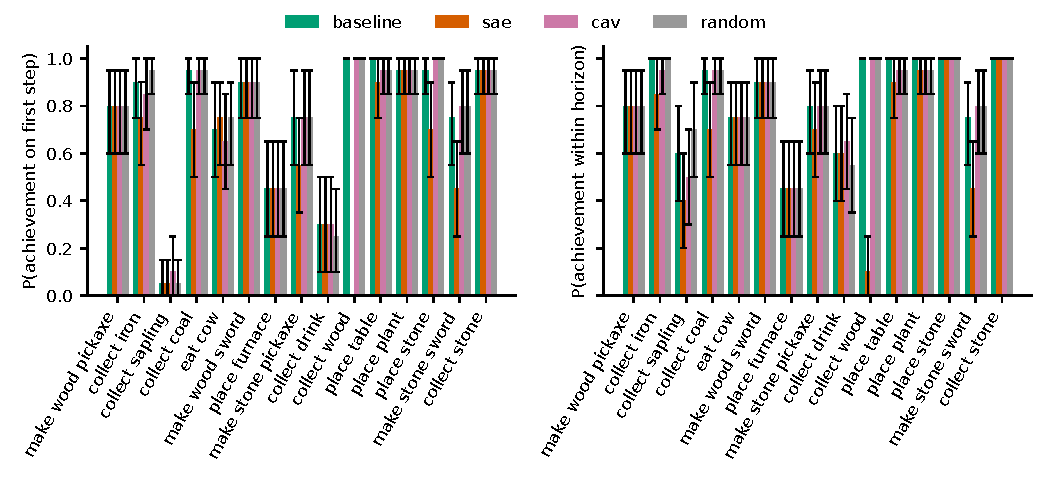
\includegraphics[width=\textwidth]{figures/imagination.pdf}
\caption{\textbf{Read--write asymmetry inside imagination.} Change in the probability that a concept's detector code is sampled during 12-step imagination---first step (left) and anywhere in horizon (right)---under SAE-direction (blue), CAV-direction (magenta) and random-direction (grey) ablation, relative to baseline; $n{=}20$ rollouts. Shaded band is the baseline 95\% CI. The matched SAE direction selectively lowers achievement (dramatically for \achname{collect\_wood}); CAV and random stay within noise.}\label{fig:imag}
\end{figure}

\textbf{The asymmetry survives multi-direction ablation.} Single-direction removal is a weak instrument against redundant codes~\cite{ravfogel2020inlp}. Generalising to a rank-$r$ orthonormal subspace $h'=h-QQ^\top h$ (Methods), the matched SAE-feature stack accumulates causal weight with rank---mean $\Delta\log P$ climbs $0.51\to2.57$ nats for $r{=}1\to16$ (up to $+6.3$ for \achname{collect\_coal})---whereas a matched CAV subspace saturates near $0.5$ and even declines ($0.48\to0.32$), an $\approx 8\times$ gap at $r{=}16$ (Fig.~\ref{fig:subspace}A). Yet a probe re-fit after projecting out the rank-16 CAV subspace still decodes at AUROC $\approx 0.999$ (Fig.~\ref{fig:subspace}B): the decodable information is massively redundant, distributed far outside any low-rank CAV span. Direct logit attribution corroborates the writing role---the SAE direction's mean absolute contribution to its detector code's logit is $0.31$, against $0.08$ (CAV) and $0.01$ (random), and is detector-specific (Methods). In this agent, then, dictionary directions are substantially more causally implicated than probe-derived directions---individually and as rank-$r$ subspaces---even though the probe-decodable information is the more redundant of the two.

\begin{figure}[t]
\centering
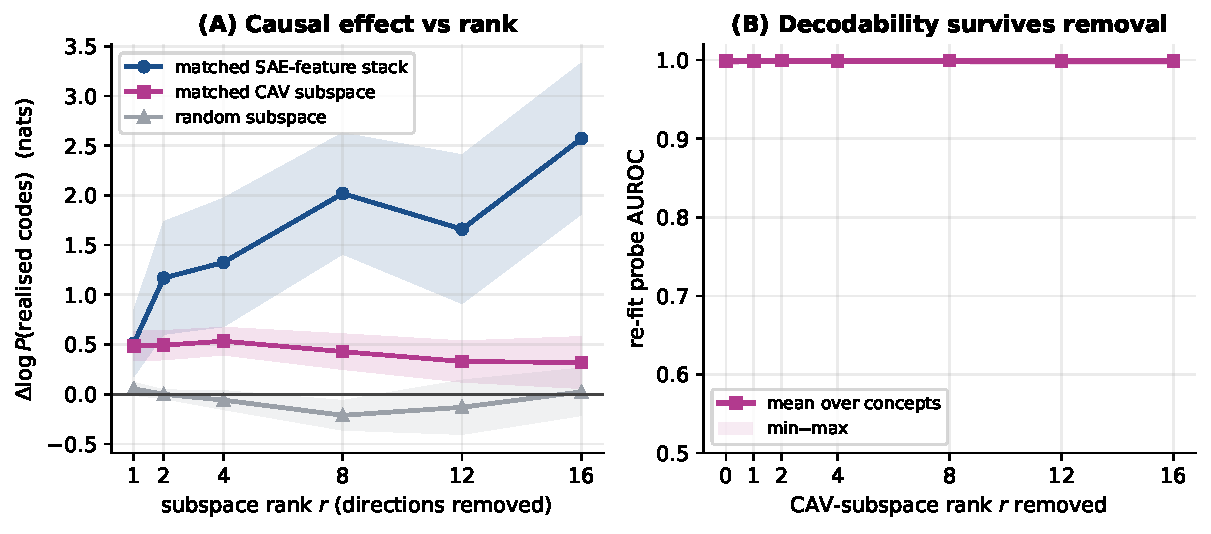
\includegraphics[width=\textwidth]{figures/subspace_ablation.pdf}
\caption{\textbf{Multi-direction ablation.} \textbf{(A)} mean $\Delta\log P$ of the realised codes (over eight dominant concepts; band $\pm$SEM) when a rank-$r$ subspace is projected out at block~1: the matched SAE-feature stack climbs with rank, the matched CAV subspace saturates ($\approx 8\times$ smaller at $r{=}16$), random is inert. \textbf{(B)} a probe re-fit after removing the rank-$r$ CAV subspace still decodes at AUROC $\approx 0.999$---the decodable information is redundant and, in this agent, is not what most drives the prediction.}\label{fig:subspace}
\end{figure}

\subsection{Next-code prediction is quasi-Markovian}\label{sec:res-trace}
Localising the causal signal by activation patching---restoring clean activations one (block, timestep, token-type) cell at a time into a corrupted run (Methods)---the picture is strikingly concentrated (Fig.~\ref{fig:trace}). Patching historical cells restores almost nothing (mean $|{\le}0.04|$ over the earliest 15 steps); at the final step the action token is the largest carrier (restoration $0.46$--$0.58$), with the latent tokens dominant for two of four concepts. Next-code prediction is computed from the current step's action and frame, not from transformer memory of the preceding twenty steps---a third line of evidence, after the \textsf{frame\_emb} control and the gap-3 ablation recovery, for the same conclusion.

\begin{figure}[t]
\centering
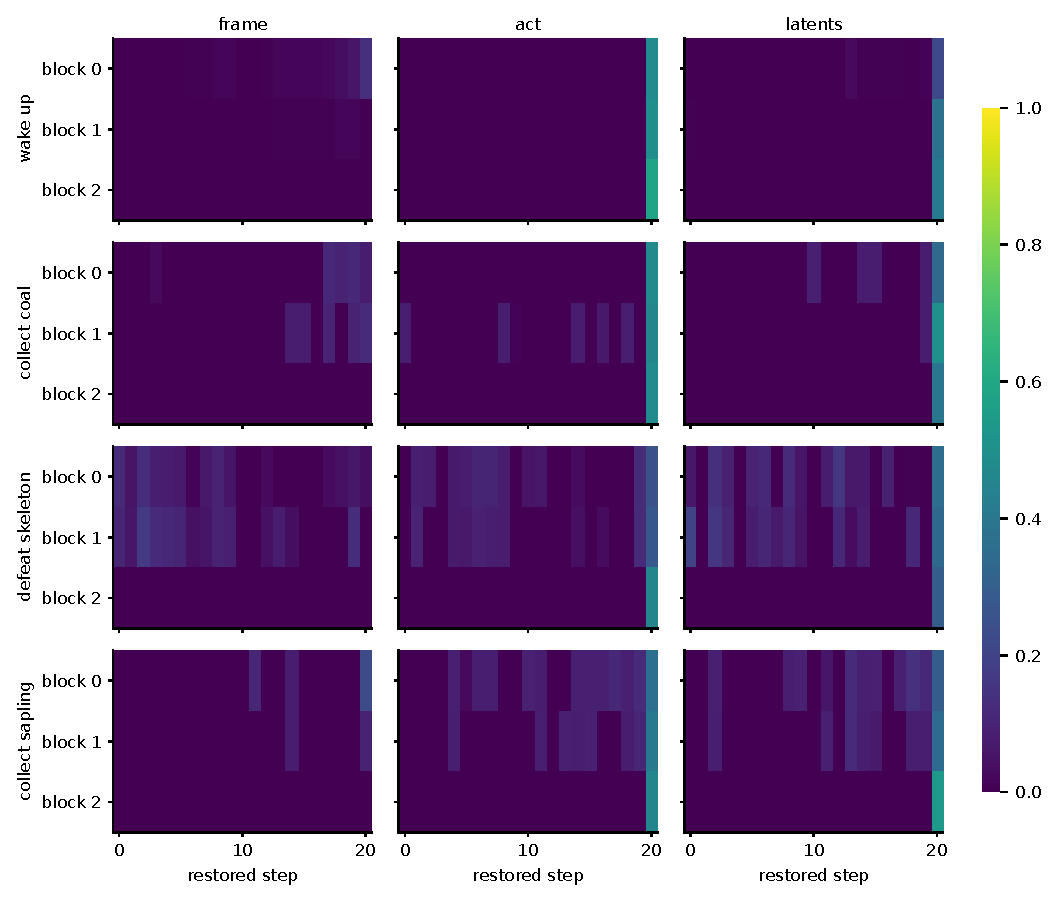
\includegraphics[width=\textwidth]{figures/causal_trace.pdf}
\caption{\textbf{Causal tracing.} Mean restoration of unlock-code prediction when clean activations are patched into a corrupted run, per (block $\times$ timestep) cell, for frame, action and latent token positions (columns) and four concepts (rows). Restoration concentrates at the final timestep on the action and latent tokens; historical cells restore essentially nothing.}\label{fig:trace}
\end{figure}

% ===================== DISCUSSION (no subheadings) =====================
\section{Discussion}\label{sec:discussion}
The audit resolves into a single spine---\emph{decode, write, drive}---with an empirical dissociation at each seam. Supervised probe directions decode concepts at near-perfect AUROC but are not what the model writes through; an unsupervised dictionary direction is (decode without write). Yet that dictionary direction, ablated, suppresses an event's code without changing the agent's imagined behaviour or return (write without drive). Crucially the two gaps are not separate findings that happen to agree with the rest; they are one fact---a quasi-Markovian model---seen at three levels. Causal tracing shows next-code prediction is computed from the current step's frame and action, not from twenty steps of memory, so suppressing a code at step $t$ cannot constrain step $t{+}k$, which re-derives the concept from its own frame---where the HUD still renders it and the convolutional encoder re-injects it. The same mechanism therefore produces the write--drive non-cascade (behaviour), the gap-3 ablation recovery (single-step prediction), and the HUD shortcut (decodability): one cause, three readouts. The functional anatomy follows: the delta codes are the event vocabulary (context-aware delta conditioning, not quantization per se, drives their specificity); the convolutional encoder carries persistent state because the environment renders it on screen; the transformer's distinctive contribution is anticipation; and the sparse dictionary directions, more than the best-decoding directions, are what it writes through---though even they do not gate behaviour.

Two methodological lessons are cheap to adopt and did the heaviest lifting. First, the input-encoder probe as a shortcut control: without it we would have reported, wrongly but at AUROC $0.98$, that the transformer tracks episodic state. Second, the double contrast in ablation (matched vs ordinary moments $\times$ matched vs random directions), without which single-direction ablations are uninterpretable. More broadly, descriptive and informational evidence---association tables, probe accuracies, concept geometries---should be treated as hypothesis generators for intervention, not as findings about mechanism~\cite{belinkov2022probing,atrey2020saliency}. The read--write asymmetry has a plausible mechanism: a probe is free to exploit any correlated signal across many directions, whereas a TopK autoencoder must reconstruct the activation from few directions, so its decoder columns span the signal the computation consumes~\cite{gao2024topk,elhage2022superposition}; recent reports that linear concept-removal and steering carry unintended effects~\cite{gumbelcf2025,goyal2025causal,propprobes2025} are consistent with this. We cannot fully exclude geometric alternatives: SAE decoder columns might align with higher-variance directions of the residual stream, so projection could perturb predictions more for reasons of geometry than of mechanism, and causal interventions can in general push activations off the model's natural distribution~\cite{grant2026divergent}. The controls argue against a pure-variance account---a random unit direction of the same norm is inert, and the effect is concentrated at unlock rather than ordinary moments---but they do not settle it; a definitive test would match candidate directions on explained variance and would intervene by steering as well as ablation, both of which we leave to future work. An independent, concurrent audit of transformer \emph{video} world models reports the same pattern in a very different setting---motion direction is linearly decodable yet steerable only through a coordinated high-dimensional subspace rather than a single low-rank direction~\cite{joseph2026physics}---suggesting the decode-versus-drive gap is not unique to this agent. The quasi-Markovian finding is double-edged: it shows economy (the model does not duplicate on-screen state in attention) but implies Crafter underuses the 21-step context, so environments with genuinely hidden state would better exercise---and let one audit---the transformer's memory. It also carries a concrete warning for model-based control: the same shortcut that makes the model sample-efficient lets imagined steps re-derive state from the rendered frame rather than from a causal history, so its rollouts can contain causally impossible transitions---a wooden pickaxe crafted from wood that was never collected---and planners that optimise against imagined achievement or reward signals on this class of model should validate them against the simulator.

\textbf{A partially observed control.} We test this directly by training a second agent (identical code, hyperparameters and seed) on a no-HUD Crafter variant that zeroes the on-screen inventory and vitals, making them hidden state (Methods; Supplementary Fig.~S5). The agent is markedly handicapped (mean return $16.2\to9.7$), and the internal signatures shift as predicted. Causal tracing now reaches far further into history---mean restoration on historical cells rises $\approx\!5\times$ ($0.03\to0.15$) while the final-step mass is unchanged---so next-code prediction de-Markovianises exactly where hidden state should force it, and the event vocabulary weakens (mean best detector lift $211\times\to88\times$), indicating that part of the with-HUD codes' specificity rode on HUD-counter increments. The input-encoder shortcut does not, however, simply disappear: \textsf{frame\_emb} cumulative-state AUROC falls only for the six concepts whose state was genuinely HUD-only (e.g.\ \achname{place\_plant} $1.00\to0.66$, \achname{collect\_sapling} $1.00\to0.73$), while world-persistent achievements---placed objects, gathered materials, tools---stay near $1.0$ because they leave visible marks in the scene. The behavioural cascade cannot be repeated on this agent for the same reason: handicapped, it almost never imagines the downstream wooden-tool tier (baseline imagined-unlock rate $\le0.05$, versus $0.80$ with the HUD), so no behaviour remains for a lesion to break---and zeroing the HUD anyway leaves wood visible in the world view, a second frame-carried route a wood-code lesion would not sever. The control therefore remains essential, now guarding against a second, world-persistence confound; and the transformer still does not make the hidden state linearly decodable from its blocks (a block out-reads \textsf{frame\_emb} on only $1$ of $17$ concepts), so it draws on history \emph{causally} without exposing it to a probe---consistent with the read--write asymmetry.

Our audit covers one agent, one seed, one environment. Most importantly, every quantitative claim rests on a single training seed; replicating the headline results---the event-specificity of the codes and its delta-trick origin, the HUD shortcut, and the SAE-versus-CAV intervention gap---across several independently trained seeds is the single most important next step, and we report effect sizes and controls precisely to make that replication straightforward. The central HUD finding also bounds how much the transformer must remember; we therefore additionally audited a partially observed (no-HUD) variant (above), though broader environments with structurally hidden state remain to be tested. We extend the read--write asymmetry from single directions to rank-16 subspaces, but larger subspaces, other layers and iterative nullspace projection remain; our sufficiency (steering) test was only weakly positive; and the imagination outcome measure shares provenance with the feature-selection statistic, a circularity we flag throughout. With those caveats, the discipline the audit recommends generalises: in world models as in language models, interpretability claims should climb from description to intervention before they are believed.

% ===================== METHODS =====================
\section{Methods}\label{sec:methods}

\subsection{The \deltairis{} agent}\label{m:agent}
\deltairis{}~\cite{deltairis2024} comprises a tokenizer, a transformer world model and a CNN--LSTM actor--critic trained jointly on imagined trajectories. The tokenizer encodes a transition $(x_t,a_t,x_{t+1})$, $x\in\mathbb{R}^{3\times64\times64}$, by stacking both frames and an action-embedding channel through a convolutional encoder; the latent is reshaped into a $2\times2$ grid of slots, each vector-quantised~\cite{vqvae2017} against a shared codebook of $C{=}1024$ entries ($d{=}64$, cosine), giving four codes $\mathbf{c}_t\in\{0,\dots,1023\}^4$. The decoder reconstructs $x_{t+1}$ from $(x_t,a_t,\mathbf{c}_t)$, so the $40$ bits of code need carry only the transition's residual novelty. Each timestep contributes a six-token block (frame embedding, action embedding, four code embeddings) to a causal transformer ($L{=}3$ blocks, 8 heads, $d_{\mathrm{model}}{=}512$, context $21$ timesteps). Three MLP heads read fixed intra-block positions: \texttt{head\_rewards}/\texttt{head\_ends} at the action position; \texttt{head\_latents} at positions 1--4, predicting the four codes autoregressively (Supplementary Fig.~S2). During imagination, codes are sampled from \texttt{head\_latents}, decoded to a frame and fed back; the actor--critic acts on decoded frames. Figure~\ref{fig:overview} overviews the model and our instrumentation.

\subsection{Agent training and instrumented rollouts}\label{m:train}
We trained one agent with the public reference implementation and unmodified Crafter hyperparameters ($1{,}000$ epochs; $10^7$ steps; seed 0) on one NVIDIA H200 ($\approx 8.7$ days). Over 500 fresh episodes the mean return is $16.20$ (s.d.\ $1.62$) with $17.1$ achievements unlocked, within one seed-level s.d.\ of the published $17.8\pm1.4$~\cite{deltairis2024}. Coverage is dense (18 of 22 achievements unlock in $\ge 73\%$ of episodes); \achname{collect\_diamond}, \achname{eat\_plant} and the two iron tools unlock too rarely and are excluded from per-achievement statistics. The training pipeline discards environment info, so we re-rolled the frozen agent recording, per step, the four codes, action, reward and 22-bit achievement state (whence just-unlocked indicators): 500 episodes ($294{,}916$ steps) for association statistics, and 150 episodes ($81{,}919$ steps) with stored frames for activation extraction.

\subsection{Association statistics}\label{m:assoc}
For every (slot, code, achievement) cell with co-occurrence support $\ge 5$ we compute $P(u^i\mid c^k{=}j)$, lift over base rate, and an exact binomial $p$-value; $190$ of $431$ cells survive Bonferroni correction. Codebook utilisation is computed by re-encoding the full buffer.

\subsection{Isolating the delta trick}\label{m:delta}
We train two baselines on the same buffer and run the identical code$\to$achievement analysis over a common 150-episode set: a \emph{frame-only ablation} (the \deltairis{} convolutional backbone, $1024$ codes, four tokens, but the encoder sees only $x_{t+1}$ and the decoder reconstructs from codes alone) and the \emph{original IRIS} tokenizer ($512$ codes, 16 tokens/frame, no action). On a common 8{,}192-transition held-out batch, matched-protocol reconstruction gives PSNR $36.7$ (\deltairis{}), $18.4$ (frame-only) and $22.5$ (IRIS) with codebook perplexity $80.7$, $48.5$ and $109.2$; \deltairis{}'s lower error is expected, as it reconstructs the residual given $(x_t,a_t)$ (Supplementary Table~S3).

\subsection{Probes and concept activation vectors}\label{m:probes}
For each timestep we extract seven representations: \textsf{raw\_codes} (mean of four codebook vectors); \textsf{frame\_emb} (CNN over $x_t$); \textsf{wm\_latents\_emb} (the model's code embedding); and the four transformer stages (blocks 0--2 and the final post-norm state), each summarised by averaging the four latent-token positions. Logistic-regression probes for 47 targets (action; instantaneous, and within-5-step reward; just-unlocked and cumulative achievement indicators) use episode-disjoint 80/20 splits. CAVs are the standardised weight vectors mapped back to raw activation space; complementary non-linear methods instead read information from activations by sampling inputs that produce matching activations and causally verifying it~\cite{huang2024inversionview}. For the HUD margin we bootstrap the held-out AUROC ($B{=}1000$) and report paired CIs on the \textsf{frame\_emb}$-$block difference per concept (Supplementary Table~S4).

\subsection{Sparse autoencoder}\label{m:sae}
A TopK SAE~\cite{gao2024topk} ($M{=}2048$ features, $k{=}16$, tied init, unit-norm decoder) is trained on the $81{,}919$ block-1 summary activations (80 epochs, Adam, lr $5{\times}10^{-4}$). Each feature is labelled by best-matching achievement (lift within its top activation quartile), CAV (decoder--CAV cosine) and code; five features satisfy strict triple-corroboration. A robustness sweep over widths $M\in\{1024,2048,4096\}$, sparsities $k\in\{8,16,32\}$, two seeds and four layers gives FVU $0.036$--$0.054$ with $\le 28$ dead features; detector features reappear as each variant's own top detector (mean matched cosine $0.63$) (Supplementary Table~S5). Residual-stream SAEs transfer to vision transformers~\cite{kim2025rrm}; their privileged interpretability over simpler bases is debated~\cite{ye2025kvmem}, and a complementary route obtains interpretable circuits via weight sparsity rather than activation-sparse dictionaries~\cite{gao2025weightsparse}.

\subsection{Projection ablation, steering and the empirical null}\label{m:ablation}
At the block-1 output we project out a unit direction $\hat d$ (matched SAE decoder column, matched CAV, or random) at the four latent positions of a chosen step, and measure $\Delta\log P$ (baseline$-$ablated) of the four realised codes at the target step, over $n{=}80$ moments per cell (gap 0 and gap 3) with $95\%$ bootstrap CIs. Projection is one of several ablation operators; optimal ablation instead substitutes a component's loss-minimising value and can yield tighter component-importance estimates~\cite{li2024optimalablation}. For the empirical null we draw $R{=}50$ random directions and report the matched effect's percentile/$z$. Inside imagination we burn in 8 real steps, force the real action, then sample 12 steps with $\hat d$ continuously projected out, scoring detector-code occurrence ($n{=}20$). Steering replaces projection with addition ($h\mathrel{+}=\alpha\hat d$, $\alpha$ up to 8 RMS) from ordinary moments (Supplementary Table~S7).

\subsection{Multi-direction subspace ablation}\label{m:subspace}
We replace single-direction projection with removal of a rank-$r$ orthonormal basis $Q\in\mathbb{R}^{D\times r}$, $h'=h-QQ^\top h$, sweeping $r\in\{1,2,4,8,12,16\}$ for eight dominant concepts. The matched CAV subspace is a Gram--Schmidt basis over the concept's CAV and its nearest tech-tree-neighbour CAVs; the SAE-feature stack is its top-$r$ decoder columns by lift; the random subspace is a QR of Gaussian noise. We measure single-step $\Delta\log P$ (gap 0) and, separately, the AUROC of a probe re-fit on activations after projecting out the rank-$r$ CAV subspace; unsupervised methods also exist for discovering causally meaningful, non-basis-aligned subspaces directly~\cite{huang2026subspaces}, as do supervised interchange-intervention methods that align learned subspaces with causal variables~\cite{wu2023das}.

\subsection{Direct logit attribution}\label{m:logit}
For each concept we attribute the \texttt{head\_latents} logit of its top detector code to a candidate direction by gradient$\times$activation, $\sum_{\text{latent pos}}(\partial\,\mathrm{logit}/\partial\langle h,\hat d\rangle)\langle h,\hat d\rangle$, with a random other code as control; we report mean absolute detector attribution and detector-vs-control specificity over 18 concepts (Supplementary Table~S8).

\subsection{Causal tracing}\label{m:trace}
For each unlock window (clean) we build a corrupted run from an ordinary window of the same episode, restore clean activations one (block, timestep, token-type) cell at a time (token types: frame, action, latents), and measure restoration $(\ell_{\mathrm{patched}}-\ell_{\mathrm{corrupt}})/(\ell_{\mathrm{clean}}-\ell_{\mathrm{corrupt}})$ over $n{=}24$ window pairs per concept, following activation-patching best practice in the corruption scheme and restoration metric~\cite{zhang2024patching}; this patching-and-knockout methodology was popularised by end-to-end circuit discovery in language models~\cite{wang2023ioi}, and related causal-mediation analyses localise behaviour-carrying directions~\cite{vig2020causal,todd2024functionvectors}.

\subsection{Partially observed (no-HUD) control}\label{m:nohud}
To separate the HUD shortcut and quasi-Markovian dynamics from environment-specific artefacts, we trained a second agent with identical code, hyperparameters and seed on a Crafter variant whose observations zero the heads-up-display region (inventory and vitals), rendering those quantities hidden state while leaving the world view, rewards and terminations untouched. We re-ran the probe, mutual-information and causal-tracing stages on this agent and compared per concept against the with-HUD agent; the agent's mean return falls from $16.2$ to $9.7$ over 500 evaluation episodes (Supplementary Fig.~S5).

\subsection{Behavioural cascade through the tech tree}\label{m:cascade}
Because the actor--critic acts on the decoded frames inside imagination, a residual-stream lesion can in principle change the agent's behaviour, not only its next-code distribution---a test the sequence-model analogues cannot run, having no downstream policy. From \achname{collect\_wood} unlock moments we run closed-loop imagination ($n{=}40$ moments; burn-in 8, horizon 12; the actor--critic selects each action from the decoded frame) under baseline, SAE-$f_{187}$, wood-CAV and random projection at block~1, recording per rollout the imagined return (sum of the reward head) and, for every achievement, whether its detector codes are sampled within the horizon. We read the outcome against Crafter's tech tree (\achname{collect\_wood}~$\to$~\{\achname{place\_table}, wooden tools\}~$\to$~\achname{collect\_stone}~$\to$~stone tier), a pre-specified causal graph that provides a built-in correctness criterion (Supplementary Fig.~S6).

\backmatter

\bmhead{Supplementary information}
Supplementary Information (Figs.~S1--S4, Tables~S1--S6) accompanies this article. Interactive HTML artefacts for every experiment are produced by the released code.

\bmhead{Acknowledgements}
Experiments were carried out on the High End Computing facility at Lancaster University.

\section*{Declarations}
\noindent\textit{Received:} \texttt{[date]}; \textit{Accepted:} \texttt{[date]}.
\begin{itemize}
\item Funding: Not applicable.
\item Conflict of interest: The author declares no competing interests.
\item Ethics approval: Not applicable.
\item Data availability: Result summaries are included with the code repository; the trained checkpoint and replay buffer ($\sim$170\,GB) are available from the author on reasonable request.
\item Code availability: All analysis code, Slurm pipelines and figure scripts are at \url{https://github.com/rxailab/delta-iris-interpretability}.
\item Author contributions: R.X.\ designed and performed the experiments, analysed the results and drafted the manuscript. R.J.\ contributed to conceptualisation, interpretation of results, supervision, and manuscript review and editing.
\end{itemize}

\bibliography{sn-bibliography}

\end{document}
